% An Applied Mathematics/Biology Thesis
% By Jonathan Niles

\documentclass[phd,tocprelim]{cornell}

% packages
\usepackage{fixltx2e}
\usepackage{geometry}
\usepackage{graphicx}
\usepackage{amsmath,amssymb}
\usepackage{tabu}
\usepackage{longtable}
\usepackage{booktabs}
\usepackage{ifpdf}
\usepackage{appendix}
\usepackage[hidelinks]{hyperref}
\usepackage{natbib}
\usepackage[toc]{glossaries}

% cite package, to clean up citations in the main text. Do not remove.
%\usepackage{cite}

% Remove comment for double spacing
%\usepackage{setspace}
%\doublespacing

% Set tolerance for box model
\tolerance=9999

% New Commands, refreshers
%\renewcommand{\caption}[1]{\singlespacing\hangcaption{#1}\normalspacing}
\renewcommand{\topfraction}{0.85}
\renewcommand{\textfraction}{0.1}
\renewcommand{\floatpagefraction}{0.75}

% Make cornell style
\normalspacing\setcounter{page}{1}\pagenumbering{arabic}
\pagestyle{cornell} \addtolength{\parskip}{0.5\baselineskip}

% LongTabu Fix
\AtBeginEnvironment{longtabu}{\tiny}{}{}   %% change all longtabu content to foot note size

% Make a glossary using the glossaries package
\makeglossaries%

%
% Actual Document Starts here!
%
\begin{document}

% import titlepage
% title.tex

\title{Crumble into Cancer: Fragility and Disease in Human Genome Architecture}
\author{Jonathan Niles}
\conferraldate{April}{2015}
\degreefield{Bachelor of Arts}


%\maketitle
%\makecopyright

%\contentspage
%\tablelistpage
%\figurelistpage

% introduction.tex

\chapter{Introduction}

What causes the genome to break?  The human genome is a six billion nucleotide string that encodes the
the vast instruction set for the cells growth, function, and death.  All possible expression patterns are
encoded in this instruction set, yet particular cell types arise when the instructions are compiled differently
during differentiation.  Modern cancer research indicates the establishment of this epigenetic landscape
determining cell fate may play a strategic role in cancer genesis.

We investigate the mechanical and structural changes during differentiation in order to establish an
architectural link between nuclear topology and the probability of developing cancerous lesions.  We
assume that mutations occurring frequently in specific cancers are based on the epigenetic architecture
of the original cell type.  Using human embryonic stem cells and lung fibroblasts, we propose that
topological changes similar to those that establish patterns of differentiation are responsible for
introducing lesions seen in many cell type specific cancers.

This thesis will proceed as follows.  First, the analytical tools to perform data analysis on genomic
data sets is introduced.  These tools include iterative normalization of chromatin contact maps, eigenvalue
decomposition, and an algorithm to detect topologically associating domains from normalized contact maps.
A literature review of chromatin architecture is presented to provide a strong biological foundation from which
to interpret results.  The methods for data acquisition and processing is described, and we conclude with a
discussion of the results and propose areas of further investigation and improvement.

% math.tex

\chapter{Mathematical Preliminaries}

To extract biologically meaningful information from large data sets, researcher rely heavily on mathematical insights which
guarantee run time estimates, bounds on the problem domain, or interpretation of significance.  While studying the relationship
between chromatin topology and fragility, we leveraged several statistical and linearly algebraic tools.  The following section
will explain the underlying mathematical notions behind the algorithms, the biological rationale, and an interpretation of their
results.  We assume the reader is familiar with the mechanics of linear algebra, an elementary course in statistics, and numerical
analysis.  The reader is heartily encouraged to consult the references to gain a more complete understanding than possible to
present here.

\section*{Normalization of Chromatin Contact Maps}

The entry point for topological analysis begins with a chromatin \gls{contact map}.  The experimental procedure generating a chromatin
contact map, called a Hi-C experiment, is described in detail in Chapter 3.  For now, we will attempt to motivate our
analysis with a simple thought experiment.

Suppose that one wished to record the conformation of a string folded randomly on a surface.  In particular, suppose we focus on intersections
where two strands cross or lie in close proximity.  One possibility would be to place a one-dimensional coordinate system on the string, say
$0 \leq  x \leq  L, x \in \mathbb{N}$.  Since we are interested in overlapping regions, we refer to the region $X_i = \left[ x_{i}, x_{i+1}\right]$
as a bin.  We can record overlapping regions as pairs $(X_i,X_j)$, where position $X_i$ is in close proximity to position $X_j$.  The 
coordinate pairs naturally form a graph, which we represent computationally as a matrix $\matr{O}$.  As $L \rightarrow \infty$, the
resolution of the matrix increases (bin sizes become smaller), and precise interactions on a smaller scale can be differentiated.
Figure~\ref{fig:string} is an example of one such diagram.

\begin{figure}[thb]
  \centering
  \caption{Example: Interactions on a String}
  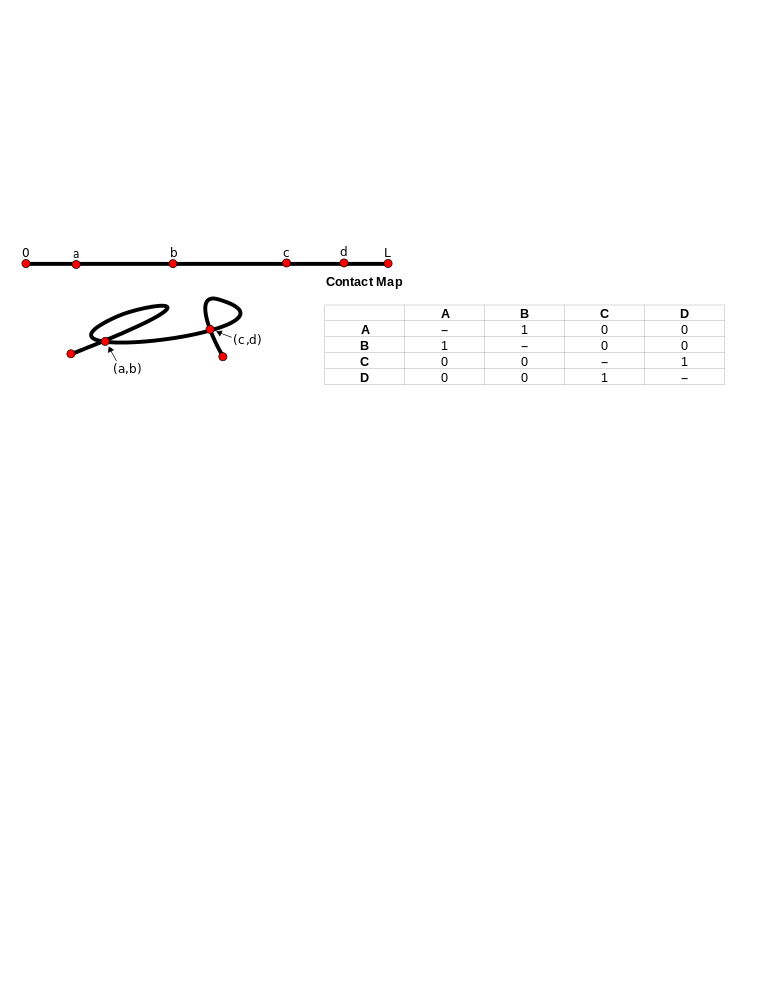
\includegraphics[width=\textwidth]{figures/mathematics/strmtx}\label{fig:string}
\end{figure}

The data structure produced by a Hi-C experiment is identical in spirit to the model developed in our thought experiment.  However, instead of
interactions occurring on a single string, the human genome consists of 24 independent chromosome `strings'.  Furthermore, interaction maps are
generated from populations of cells, yielding millions of copies of each genome.  With this in mind, we propose the following definition:

\begin{defn}
  A chromatin contact map $\matr{O}$ is a symmetric $N \times N$ matrix.  Each cell or bin $O_{ij}$ contains the number of observed contacts
  between regions $i$ and $j$ on the genome.  The contact map is a measure of the contact probability between loci on a genome-wide scale.
\end{defn}

Contacts are recorded by binning the genome into equally sized intervals and considering the pairwise interactions between each bin.
Typically, bins are ordered by increasing genomic coordinates, from the first bin of chromosome 1 to the last bin of chromosome X.
Depending on data quality, bin sizes range from tens of kilobases to megabases.

The critical step of any data analysis pipeline is data \gls{normalization}, which removes experimental biases and noise.  Coupled with quality
control measurements and experimental replicates, normalization also establishes a level of reproducibility.
Several methods exist to normalize contact maps.  Tanay and Yaffe were among the first researchers to undertake a statistical analysis of the
Hi-C experiment in 2011 \citep{yaffe2011}.  They identify several sources of systematic experimental bias in the Hi-C assay and propose a
probabilistic background model that computes the probability of \glspl{trans contact} and \glspl{cis contact} based on regional
\gls{GC} content, fragment length, and genome mappability.  Corrected contact maps are calculated by solving the maximum-likelihood model
parameters on model contact maps, which are then applied to the experimentally derived contact maps.  The mappings
achieved using Tanay and Yaffe's methods provide robust reproducibility between replicates and experiments by considering
\glspl{trans contact} and \glspl{cis contact} separately \citep{yaffe2011}.  This requirement renders their analysis computationally
intensive, prompting further research into simpler methods for Hi-C analysis.

Alternative methods have been developed to normalize contact maps.  Hu and colleagues propose a method `HiCNorm' based on Poisson
regression and achieve a $9000$-fold speed increase compared to Tanay and Yaffe's method \citep{hu2012}.  Recently, Ay and colleagues provide a statistical
method `Fit-Hi-C' that does not assume a particular underlying statistical distribution, instead normalizing \glspl{cis contact} based on probabilistic
analysis of polymer looping dynamics \citep{ay2014}.

Imakaev and colleagues propose a normalization and analysis pipeline \gls{ICE} \citep{imakaev2012}.  We employ \gls{ICE} as the normalization
algorithm in this thesis, due to the availability of its source code\footnote{source: \url{http://mirnylab.bitbucket.org/hiclib/}} and good
performance.  In the following section, we will discuss their algorithm in detail.

\subsection*{\glsentryfull{ICE}}

In pursuit of the true contact probability for each genomic region, \gls{ICE} makes a critical observation that the bias matrices determined by
Yaffe and Tanay \citep{yaffe2011} can be successfully reproduced ($r = 0.99$) as a product of biases $B_i \times B_j$.  This observation leads
immediately to the following proposition

\begin{prop}
  Given the assumption of factorizable biases, the expected contact frequency $\varepsilon_{ij}$ for every pair of regions $(i,j)$ can
  be written as $\varepsilon_{ij} = B_{i}B_{j}T_{ij}$, where $B_i$ and $B_j$ are biases and $T_{ij}$ is the sought matrix of relative contact
  probabilities, normalized as $\sum_{i, i \neq j, j \pm 1}T_{ij} = 1$.  The normalized contact map is give as
  $T_{ij} = \frac{\varepsilon_{ij}}{B_{i}B_{j}}$.
\end{prop}

The authors note that this normalization procedure results in `equal visibility' regions across the entire genome and maps which are
comparable between Hi-C data sets.  They propose the following algorithm to obtain the biases $B_i$ and `true' relative contact probabilities
$T_{ij}$.

\begin{algorithm}[H]
  \KwData{A matrix of observed interactions $O_{ij}$}
  \KwResult{A matrix of relative contact probabilities $T_{ij}$ and bias vector $B_i$}
  Initialize $W^{0}_{ij} = raw contact matrix$; $B^0 = 1$; $k = 1$\;
  \While{$\abs{B^{k+1} - B^{k}} < \delta$}{%
    $S_i = \sum_{j}W^{k}_{ij}$\;
    $\mean{S_i} = \frac{1}{n}\sum_{i = 1}^{n}S_i$\;
    $\Delta{}B^k_i = \frac{S_i}{\mean{S_i}}$\;
    $W^{k+1}_{ij} = \frac{W^k_{ij}}{\Delta{}B^k_i\Delta{}B^k_j}$\;
    $B^{k+1}_i = B^k_i \dot \Delta{}B^k_i$\;
    $k = k + 1$\;
  }
  \caption{Iterative Correction}
\end{algorithm}

It is not apparent that this algorithm is correct or even converges.  To gain an intuitive understanding of the solution, let us investigate a
simpler proposition.  Suppose that, instead of defining $O_{ij}$ to be the matrix product $B_{i}B_{j}T_{ij}$, we consider the counts
in $O_{ij}$ are the expectation of some multinomially distributed random variable $X_{ij}$, where $E[X_{ij}] = NB_{i}B_j$ for some
constant $N$ and vector $B$ whose cumulative sum is 1 ($\sum_{i}B_i = 1$).  In this formulation, we relax our criteria such that each cell
$O_{ij}$ is independent and distributed according to $B$.  The count of cell $i,j$ is given by the probability

\begin{align}
  \label{eqn:probmodel}
  \begin{split}
    p_{ij} &= NB_{i}B_{j}
    \\
    \log{p_{ij}} &=  c + u_i + u_j - Z
  \end{split}
\end{align}

where $c = \log{N}, u_i = \log{B_i}, u_j = \log{B_j}$, and $Z (= c)$ is a normalization factor to ensure that $\sum p = 1$.  This type of
model is called a \gls{log-linear} or \gls{toric model}.  $p$ is an observation from some distribution $p \sim \mathcal{f}(X)$.  The challenge to
parameterize the model and fit the model to the observed map.  The problem one of \gls{MLE}: what are the maximum likelihood parameters
that best fit the model to the observed data?  Fortunately, methods and their convergence properties for solving \glspl{MLE} have been extensively
studied in the literature \citep{fienberg2012, pachter2005}.

% TODO
In the realm of statistics, the contact matrix, together the vector sums of the rows and columns (margins), is called a \gls{contingency table}.  Assuming
that the margins are positive, and that the matrix cannot be permuted into block diagonal shape, Birch's theorem guarantees that there is a
unique maximum to the likelihood function \citep{pachter2005,bishop1975}.  For full details, consult Discrete Multivariate Analysis by
Bishop \citep{bishop1975}.  Furthermore, the marginal values are the \glspl{sufficient statistic} of the model.  In other words, the maximum
likelihood parameters for this data is given by the normalized row and column sums of the matrix \citep{pachter2005}.

With the observation that there exists a global maximum of the likelihood function, all that remains is to compute the true values by some
process.  One common algorithm is the \gls{EM} algorithm \citep{fuchs1982}.  Imakaev and colleagues employ a simpler algorithm known as \gls{IPF},
developed by Deming and Stephan in 1940, and apparently rediscovered by Imakaev's group \citep{deming1940}.  \gls{IPF} works generally by solving
the \gls{MLE} problem while leaving the margins ($p_{i+} = \sum_{j}p_{ij}$ and $p_{j+} = \sum_{i}p_{ij}$) fixed.  A proof of convergence for contingency
tables follows from Fienberg's work in algebraic geometry in 1970 \citep{fienberg1970}. %TODO explain feinburg more

Finally, we return to the \gls{toric model} we described in Eqn.~\eqref{eqn:probmodel}.  Since the log-likelihood function is concave, the \gls{IPF} algorithm first
computes the roots of the partial derivatives of the log-likelihood function and sets them to zero to solve for the global maximum.  Imakaev
and colleagues consider the likelihood function on the Poisson distribution, given by the \gls{pdf} $f(O;E) = \frac{E^{O}}{O!e^{-E}}$.  The
log-likelihood function for the Poisson distribution is given

\begin{align}
  \label{eqn:llmodel}
  LL = \sum_{ij}\left[O_{ij}\log{(T_{ij}B_{i}B_{j})} - T_{ij}B_{i}B_{j} - \log{(O_{ij}!)}\right]
\end{align}

Differentiating with respect to $T_{lm}$ and $B_m$ and setting the derivatives to zero yields

\begin{multicols}{2}
  \begin{align}
    \label{eqn:modelderivative1}
    \begin{split}
      \frac{dLL}{d\matr{T}_{lm}} = \frac{O_{lm}}{T_{lm}} - B_{l}B_{m} = 0
      //
      \frac{dLL}{dB_{m}} = \sum_i\left[\frac{\matr{O}_{im}}{B_m} - T_{im}B_i\right] = 0
    \end{split}
  \end{align}

  \break%

  \begin{align}
    \label{eqn:modelderivative2}
    \begin{split}
      T_{lm} = \frac{\matr{O}_{lm}}{B_{l}B_{m}}
      \\
      \sum_i\left[\frac{\matr{O}_{ij}}{B_{m}B_{i}} - \matr{T}_{im}\right]
    \end{split}
  \end{align}
\end{multicols}

It is clear that Eqn.~\eqref{eqn:modelderivative2} is satisfied if a solution is found for Eqn.~\eqref{eqn:modelderivative1}.  Taking the first equation together  with the
normalization $T_{ij}$ yields

\begin{align}
  \label{eqn:result}
  \sum_i \frac{\matr{O}_{ij}}{B_{i}B_{j}} = 1
\end{align}

A similar process yields that a broad class of distributions give the same result \citep{imakaev2012}.

\section*{Principal Component Analysis}

The holy grail of data analysis on high-dimensional data is dimensionality reduction --- that is, to find an accurate representation of
the experiment that need not invoke all the dimensions measured.  This is often performed as a preprocessing step to increase storage capacity
and algorithm speed.  Since experiments such as Hi-C produce data on large numbers of features, researchers must find ways to remove redundancy,
eliminate unneeded parameters and compress data sets.  One of the most popular methods is called \gls{PCA} \citep{law1987}.

Data in high dimensions are difficult to visualize and interpret.  Two common questions in data analysis are `what changed?' and `what
remained the same?' between measurements.  \gls{PCA} answers these questions by finding a representation of the data that maximizes
the \gls{variance} or variation between observations in the data set.  The output of \gls{PCA} is a transformed data set on a new coordinate
system, called components.  The \glspl{PC} are a subset of these components that capture `most' of the variation in the data set.  The researcher
must compare the calculated components to the original data set and determine which variables, or combination thereof, the components represent.

\begin{defn}[Principal Component Analysis]
  A statistical procedure that transforms a number of possibly correlated variables into a smaller number of uncorrelated variables.
\end{defn}

In practice, there are two methods used for \gls{PCA}.  The simplest to explain, but more error-prone, is the eigen-decomposition
method \citep{smith2006}.  In this procedure, for a data matrix $\matr{A}$, the eigenvalues of the covariance matrix $\matr{A}\matr{A}^T$
are computed directly as the principal components.  However, since this method requires an extra matrix multiplication, numerical
errors are more likely to be introduced during large computations. In practice, \gls{PCA} often derived in conjunction with \gls{SVD}
and we will hold to that standard here.

\begin{thm}[Singular Value Decomposition]
  Let $\matr{A} \in M_{n}(\mathbb{R})$ be given. Then there are unitary matrices $\matr{V} \in M_n$ and $\matr{W} \in M_n$, and a square diagonal
  matrix
  \[
    \matr{\Sigma} =
      \begin{bmatrix}
        \sigma_1 &        & 0        \\
                 & \ddots &          \\
        0        &        & \sigma_n \\
      \end{bmatrix}
  \]
  such that $\sigma_1 \geq \sigma_2 \geq \cdots \geq \sigma_n$ and $\matr{A} = \matr{V}\matr{\Sigma}\matr{W}^*$.  The parameters $\sigma_1$,
  $\hdots$, $\sigma_n$ are the positive square roots of the decreasingly ordered non-zero eigenvalues of $\matr{A}\matr{A}^*$, which are the
  same as the decreasingly ordered nonzero eigenvalues of $\matr{A}^*\matr{A}$.
\end{thm}

To prove that any square matrix $\matr{A} \in M_n(\mathbb{R})$ can be decomposed into singular values, we will use some matrix definitions. The
reader is reminded of the definitions of \textit{normal} $(\matr{A}\matr{A}^* = \matr{A}^*\matr{A})$, \textit{Hermetian} $(\matr{A}^* =  \matr{A})$,
and \textit{unitary} $(\matr{A}^*\matr{A} = \matr{A}\matr{A}^* = 1)$ matrices.  Further, two matrices $\matr{A}, \matr{B} \in M_n$ are said to be
\textit{unitarily similar} they are similar by a unitary matrix $(\matr{A} = \matr{U}\matr{B}\matr{U}^*)$.  We are now ready to begin the proof.

\begin{proof}[Singular Value Decomposition]
  It should be clear the matrices $\matr{A}\matr{A}^* \in M_n$ and $\matr{A}^*\matr{A} \in M_n$ have the same eigenvalues, and hence, they are
  unitarily similar.  Then there exists a unitary matrix $\matr{U}$ such that $\matr{A}^*\matr{A} = \matr{U}(\matr{A}\matr{A}^*)\matr{U}^*$.  Then

  \[
    {(\matr{UA})}^*(\matr{UA}) =
    \matr{A}^*\matr{U}^*\matr{UA} =
    \matr{A}^*\matr{A} =
    \matr{UA}\matr{A}^*\matr{U}^* =
    \matr{UA}{(\matr{U}\matr{A})}^*
  \]

  so $\matr{UA}$ is normal.  Let $\lambda_1 = \abs{\lambda_1}e^{i\theta_1}, \ldots, \lambda_n = \abs{\lambda_n}e^{i\theta_n}$ be the positive eigenvalues of
  $\matr{UA}$ in decreasing order.  Furthermore, let $\Delta = diag(\lambda_1, \ldots, \lambda_n)$, let $D = diag(e^{i\theta_1}, \ldots, e^{i\theta_n})$,
  let $\Sigma = diag(\abs{\lambda_1}, \ldots, \abs{\lambda_n})$, and let $\matr{X}$ be a unitary matrix such that $\matr{UA} = \matr{X\Delta}\matr{X}^*$.  Then
  $D$ is unitary and

  \[
    \matr{A} = \matr{U}^*\matr{X}\Sigma\matr{D}\matr{X}^* = (\matr{U}^*\matr{X})\Sigma(\matr{D}\matr{X}^*)
  \]

  If we denote $\matr{V} = \matr{U}^*\matr{X}$ and $\matr{W} = \matr{X}\matr{D}^*$, we have our desired factorization, and
  $\sigma_j = \abs{\lambda_j}, j = 1, \ldots, n$.
\end{proof}

A full proof of \gls{SVD} for rectangular matrices can be found in Horn and Johnson \citep{horn2013}. The relationship between
\gls{SVD} and \gls{PCA} follows directly from the definition of \gls{SVD}.

\begin{thm}
  Let $\matr{A} = \matr{V}\matr{\Sigma}\matr{W}^*$ be the \gls{SVD} of an $n \times n$ dimensional matrix $\matr{A}$ and let

  \[
    \matr{C} = \frac{1}{n - 1}\matr{A}^*\matr{A}
  \]

  be the covariance matrix.  The eigenvectors of $\matr{C}$ are the same as the \textnormal{right singular vectors} of
  $\matr{\Sigma}$.
\end{thm}

\begin{proof}
  Compute
  \[
    \matr{A}^*\matr{A} =
    \matr{V\Sigma}\matr{W}^*\matr{W\Sigma}\matr{V}^* =
    \matr{V\Sigma\Sigma}\matr{V}^* =
    \matr{V}\matr{\Sigma}^2\matr{V}^*
  \]

  \[
    \matr{C} = \matr{V}\frac{\matr{\Sigma}^2}{n - 1}\matr{V}^*
  \]

  $\matr{C}$ is symmetric, and unitarily diagnolizable.  Hence, the eigenvectors of the covariance matrix $\matr{C}$ are the same as the
  matrix $\matr{V}$ (right singular vectors) and the eigenvalues of $\matr{C}$ can be computed directly from the singular values
  $\lambda_i = \frac{\sigma_i}{n - 1}$.
\end{proof}

The ordered eigenvectors are the \glspl{PC} we desire.  In exploratory data analysis, the variance captured by each \gls{PC} is found
by analyzing the relative sizes of the positive eigenvalues, typically in the form of a scree plot.  In the Hi-C capture experiment, Dekker
and colleagues \citep{dekker2012} focus on the component that captures genome `compartment character', the banding pattern of interactions
observed on Hi-C maps, regardless of captured variance.  In our case, the \gls{PCA} decomposition provides a measure of compartment character
for a given bin on the Hi-C map.

\section*{Detecting changes in local chromatin interaction}

\gls{PCA} is a useful technique for identifying gross differences between data sets.  For subtle changes of local chromatin structure, we appropriate a
technique developed by Dixon and colleagues \citep{dixon2012}, termed the \gls{DI}.  Intuitively, the \gls{DI} for a given region of chromatin gives the
relative `upstream' or `downstream' character of the interactions involving that particular chromatin region.

The basic premise of the \gls{DI} algorithm is simple.  For each bin along the genome, we calculate the number of upstream and downstream interactions and
assign the normalized difference ($downstream - upstream$) as the \gls{DI} for that particular bin.  The index captures the downstream or upstream bias of
a genomic region. The formulation of the directionality index is given in the supplementary methods of Dixon's paper  \citep{dixon2012}

\begin{align}
  \label{eqn:di}
  DI = \left(\frac{B - A}{\abs{B - A}}\right)\left(\frac{{(A - E)}^2}{E} + \frac{{(B - E)}^2}{E}\right)
\end{align}

where $A$ is the number of upstream reads in a given window, $B$ is the number of downstream reads, and $E$ is the expected number of interactions under
the null distribution ($\frac{A + B}{2}$).  Dixon and colleagues apply the directionality index to examine 2Mb windows upstream and downstream on a
normalized 40kb resolution contact map.  From the \gls{DI} vector, they employ a \gls{HMM} to discover X domains with prominent upstream and downstream bias.
They concluded that these domains were (not) conserved across cell types, but may represent an underlying regulatory structure in particular cell or tissue
types \citep{dixon2012}.

% bio.tex

\chapter{Biological Preliminaries}

\section*{Introduction}

Even if limited in scope to genome architecture, a satisfactory discussion relating cell state and architectural regulation would fill
volumes.  In the following chapter, we will discuss the topics and recent developments from genetics and molecular biology that most
directly relate to chromatin architecture and the implications of a shifting interaction map.  Readers are strongly encouraged
to consult a molecular biology text, such as Molecular Biology of the Cell \citep{alberts2002}, for a rich discussion of mechanism
regulating cell state and function.

The sheer complexity of the nucleus is best decomposed into a structural hierarchy with several layers of granularity: the primary
sequence of \gls{DNA} base pairs, architectural modeling proteins, transcription factors and other binding proteins, and \glspl{CT}
and other macro molecular chromatin structures.  Within these categories there are deeper layers of regulation, such as nested
organization of topological domains or alternative splicing in transcription.  Conformational changes at smaller resolutions generally
invoke targeted, local events, while genome-wide conformation shifts enable regulation on whole cell level.  This conceptual hierarchy
is useful to keep in mind when investigating the origin of gene expression changes, differentiation, or disease states.  We will
consider each of these levels in sequence.

\section*{The Nuclear Hierarchy}

It is difficult to overstate the importance of chromatin topology.  The morass of nucleic acids and proteins packed tightly inside the
nuclear envelope somehow contain all the information required for cell function and proliferation.  The central dogma of molecular biology,
outlined in the notes of Francis Crick's `Ideas on Protein Synthesis' \citep{crick1970} illustrates how information flows from primary
sequence through protein.  The central dogma therefore strongly reinforces the importance of \gls{DNA} content, readability, and expression.

\begin{figure}[b]
  \centering
  \caption{The original central dogma of molecular biology \citep{crick1970}}
  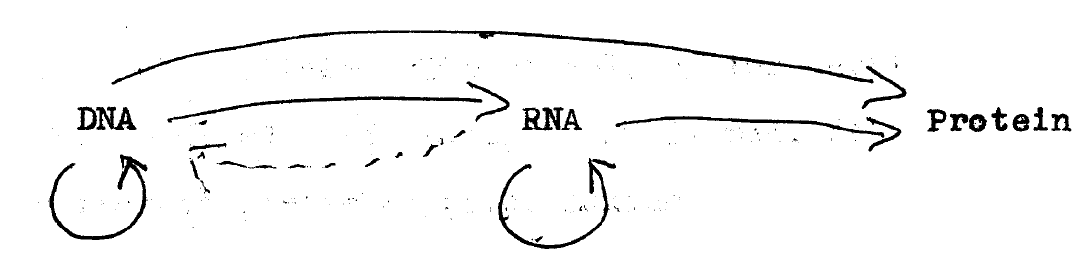
\includegraphics[width=\textwidth]{figures/biology/dogma}\label{fig:dogma}
\end{figure}

\subsection*{The Primary Sequence}

The fundamental informational unit of the cell is the \gls{nucleotide}, often called a nucleotide base or \gls{bp} when joined in a
\gls{DNA} molecule or strand.  Eukaryotic cells have a principal four character alphabet of nucleotides, distinguished by their \glspl{nucleobase}:
adenine, cytosine, guanine, and thymine.  Nucleotides are affixed to a phosphate backbone in a long, coiling polymer chain, called \gls{DNA}.  The
famous publication of the structure of \gls{DNA} in 1953 by researchers James Watson and Francis Crick demonstrates these polymers
exist in the nucleus as double helices \citep{watson1953}.  Strong hydrogen bonds between opposing nucleotides hold the double helix together
in solution.  Nucleotides are classified based on the chemical structure of there nucleobase into purine or pyridine bases; adenine and guanine are purine bases,
while thymine and cytosine are pyridine bases.  \gls{DNA} bonds form between complementary nucleotides from opposite groups: adenine and thymine form
two hydrogen bonds and guanine and cytosine form three hydrogen bonds between their bases.  Thus, one half of the helix completely
determines the other half and perturbations of this structure may lead to strand mutations \citep{alberts2002,cox2008}.

One cannot ignore the constituents of the primary sequence, particularly when considering macroscopic properties of the genome.  The nucleotide content and
order affects local sequence flexibility directly (by encoding binding sites) or indirectly (by supporting the binding of histones), and
modulates the binding of important architectural proteins \citep{travers2004}.  Although a \gls{DNA} strand is a helical structure, it is an intrinsically
flexible molecule.  A naive calculation reveals that the human genome is roughly two meters in length%
\footnote{%
  A diploid human genome consists of two copies of the $\sim3.1Gb$ DNA molecule, based off estimates from the \gls{NCBI} human genome reference build 37.
  Each base pair is assumed to be roughly $0.34\times10^{-9}m$.  The entire length is $2(0.34 \times 10^{-9})(3.2 \times 10^9) = 2.176m$.
},
yet the entire genome fits into a nuclear volume of $\sim523\mu$m \citep{marks2011}.  Loops as small as 100 bases in length have been
reported in enhancer and repressor element activation pathways \citep{wong2008}.  Furthermore, These loops can form independently of proteins
\citep{vafabakhsh2012}, indicating these loops do not impose excessive torsional strain.  Altogether, \gls{DNA}'s inherent flexibility furnishes the
foundation for complex higher order chromatin structures.

\gls{DNA} bases can also be directly modified by binding additional biochemical groups.  Cytosine undergoes \gls{DNA} methylation, also called GC methylation
to distinguish it from a histone modification of the same name \citep{bird2002}.  Methylation is an important epigenetic mark, involved in imprinting,
\gls{X-inactivation}, and maintaining heritable epigenetic states \citep{law2010}.  In mammals, \gls{DNA} methylation occurs almost exclusively along
symmetric \gls{GC} dinucleotides, and is estimated to occur at $\sim70-80\%$ of the \gls{GC} sites throughout the genome \citep{ehrlich1982,law2010}.
In the context of global chromatin architecture, \gls{DNA} methylation is thought to change chromatin conformation by recruiting histone
de-acetylaces \citep{schubeler2000}, suppressing large domains as in X-inactivation, recruiting architectural proteins directly \citep{yu2000},
and inhibiting transcription \citep{kass1997}.

\subsection*{Epigenetics And Chromatin Modeling}

How a \gls{DNA} molecule is packaged and condensed within a cell nucleus remains one of the basic questions of cell biology.  Intellectual curiosity aside,
why is it so important to unravel the chromosomal architecture?  Researcher J.C. Hansen notes, `In biology, structure is inexorably linked to function.' \citep{hansen2012}
The pursuit of an accurate \textit{\gls{in vivo}} model for \gls{DNA} and protein packaging continues to persist today, despite a legacy of experimental,
conceptual, and mathematical models.

In 1974, Kornberg discovered that chromatin contained roughly equal amounts of \gls{DNA} and protein \citep{kornberg1974}.  A year later, \citet{oudet1975}
and colleagues described the separation of chromatin into protein complexes spaced evenly on the \gls{DNA} molecule as `beads on a string' \citep{oudet1975}.
The observed beads are nucleosomes, bundles composed of a histone octamer and $\sim200$ bases (later reported to be $167$ bases) \citep{robinson2006} of
coiled \gls{DNA}. Much as the nucleotide is the fundamental unit of the genome, nucleosomes are the fundamental units of the epigenome.  Nucleosomes in
series are called a \gls{nucleosome array}.  A nucleosome consists of two components: a core particle wrapping $\sim146$ base pairs of DNA, yielding a
6 fold compaction in length, and a linker portion of varying length of $0$ to $\sim80$ base pairs.  The linker component connects adjacent nucleosomes
in a nucleosome array \citep{wu2007, hansen2012}.  These arrays are $10-nm$ in diameter, provoking them to be often called the `$10-nm$' fibers.

Despite decades of research on nucleosome arrays, their structural conformation \textit{\gls{in vivo}} remains enigmatic.  Does a higher order structure
between the $10-nm$ fiber and mitotic chromosome exist?  Nucleosome arrays and linker histones suspended in ionic solution fold naturally into a $30-nm$ fiber
\citep{tremethick2007}; however, it is unclear whether this motif forms \textit{\gls{in vivo}} and its conformation may be different in the nuclear context \citep{bian2012}.
The $30-nm$ fiber model is appealing as it readily explains the highly compacted structure of mitotic chromosomes.  To form the fiber, arrays of nucleosomes
are arranged in a solenoid or double-helix structure (for full review, see Grigoryev and Woodcock \citep{grigoryev2012}).  Whether one or both structures
are present in sub-chromosomal architectures is still an open question \citep{song2014}.  Recently, experiments using cryogenic electron microscopy
(cryo-EM) suggested an alternative fractal arrangement of $10-nm$ fibers, without invoking a higher organizational unit \citep{nishino2012,hansen2012}.
It is likely that a mixture of these organizational schemas exist in the cell.  Further research is needed to assess the biological relevance of the $30-nm$ fiber in
both interphase and mitotic chromosome structure.

The nucleosome core particle is a central actor controlling gene expression through local transcription regulation.  It is well established that nucleosomes
cause an attenuation of gene expression when present at physiological concentrations \citep{brown1984, lorch1987,laybourn1991,juan1994}. How
then does the cell maintain some genes as actively transcribed while others are silenced?  Nucleosomes regulate gene expression by regulating accessibility.
Gene expression is mediated by a confluence of protein-DNA interactions: enhancers bind to enhancer elements, polymerases to the \gls{TSS}, and polymerase
recruitment proteins line the promoter region to facilitate polymerase binding and transcription activation \citep{cox2008}.  At any protein-DNA junction,
local chromatin compaction can exclude binding by physically restricting access to the primary sequence.  This tightly packed form of DNA is called
\textit{\gls{heterochromatin}}, while open and accessible sequence is called \textit{\gls{euchromatin}}.

A critical component of gene regulation is the ability to form long range interactions between distal elements of the genome.  Enhancer or silencer elements
situated at great distances (hundreds of kilobases) from a gene promoter will form loops in the chromatin to situate that element near the target
promoter \citep{heintzman2007}.  The commonly-held view is that there are three distinctive classes of proteins facilitating gene transcription: \glspl{GTF},
promoter-specific activators, and coactivators.  \glspl{GTF} form on the promoter region, to form a \gls{PIC}, called the \gls{core promoter}.  While the
\gls{core promoter} assembly is enough to detect a basal level of transcription, often activators, proteins bound to regulatory regions upstream, downstream,
or even in neighboring genes, are recruited to the promoter region to facilitate greater level of transcription, forming long chromatin loops \citep{ptashne1997}.
Coactivators function as intermediaries in the assembly of the promoter complexes, binding both the activators and the \gls{PIC} to achieve faster throughput of
gene expression.

\subsection*{Chromosomes are organized in territories}

The highest level of genome organization is the \gls{CT} or chromosome neighborhood \citep{cremer2001}.  The hypothesis that chromosomes are segregated into
nuclear sub-volumes dates back more than 100 years \citep{cremer1993}.  The raison d'etre for these territories is not well understood; however, it is proposed
that \gls{CT} distribution in the nucleus protects the gene-rich chromosomes by localizing them to the nuclear center \citep{boyle2001, federico2006}.
\glspl{CT} create gene expression `pockets' with localized transcriptional and repair machinery \citep{bolzer2005}, and may have cell type specific positioning.

To date, there is no evidence to support a deterministic ordering of chromosomes in the nucleus.  However, there may exist certain deterministic rules to
chromosomal positioning.  In all human cell types studied, the radial position of the chromosomes is correlated with gene density and chromosome
size \citep{sun2000,bolzer2005}.  In most cell types, gene-rich chromosomes are found in the central nuclear compartment, while gene-poor
chromosomes surround the nuclear periphery, most likely to protect actively transcribed genes from mutagens that may invade the nucleus \citep{boyle2001,kozubek2005}.
However, in cell types with non-spherical nuclear shapes, chromosomal arrangements may deviate from this pattern, possibly reflecting more
specialized functions \citep{bolzer2005}.

There is strong evidence that chromosomal territories contain small decondensed regions serving as gene expression hot-spots.  Unlike bacterial chromosomes,
in which genes from the same pathway are grouped on the chromosome in units called \textit{\glspl{operon}}, eukaryotic genes are distributed seemingly randomly
throughout the genome \citep{jacob1961}.  It is well known that transcriptionally active chromatin compartmentalizes based on replication
timing \citep{ferreira1997,sadoni1999,thevenin2014}.  Moreover, recent observations reveal in order to facilitate transcription of genes in
a pathway, chromosomal territories co-localize functionally related genes with transcriptional machinery.  When considering only inter-chromosomal gene
pairs, Thevenin and colleagues observed that co-functioning genes exhibit significant local concentrations, regardless of linear distance on the primary
sequence \citep{thevenin2014}.

\section*{Experimental approaches to discern nuclear topology}

The field of molecular biology is advancing rapidly, propelled forth by a surge of automated techniques.  These so-called `\gls{high-throughput}'
methodologies enable biologists and bioinformaticians to generate massive data sets with relative ease, reliability, and efficiency.  The first
reference build of the human genome is a testament to their success \citep{hgsc2004}.  However, until recently, investigating chromosomal architecture
remained an exhaustively manual process, relying on fluorescence microscopy experiments and visual inspection by researchers.  It was not until 2003,
when Job Dekker and colleagues described a technique known as \gls{3C} that the study of nuclear architecture gained a high throughput methodology
 \citep{dekker2002}. Since then, a family of high-throughput capture techniques, most named a variation on `\gls{3C}', have been developed to interrogate
different resolutions and types of chromatin interactions (see Figure\ref{fig:captureTechniques}).

The original chromosome conformation capture technique developed by Dekker and colleagues provides an average measurement of the juxtaposition frequency
between two specific genomic loci in a cell population \citep{frase2014}.  This interaction frequency measurement is thought to be reflective of
the distance between two associated loci in genomic space.  The first extension of the \gls{3C} experiment, aptly named \gls{4C}, increased
the number of interrogated regions from two loci (one to one) to all loci interacting with a chosen target region (one to all) \citep{simonis2006}.  Most
recently, the Dekker lab extended the method further using biotinylated probes to assess contacts across the entire genome (all to all) \citep{berkum2010}.
The method, known as Hi-C, boasts the first truly global quantization of every genomic contact at a given time.

The conceptual idea behind chromosomal conformation capture is remarkably simple --- to assess nearby regions, the experimenter attempts to fuse
together molecules that are physically close, then determine the interaction partners of each segment of DNA captured in this fashion.  The
\gls{3C} procedure involves five steps.   Initially, a population of cells is cultured in an appropriate growth medium to a population size
of $\sim2.5 \times 10^7$ cells \citep{berkum2010}.  The entire population is treated with formaldehyde, a small chemical commonly used to fix both
cellular samples for microscopy experiments and large specimens for organismal analysis.  Formaldehyde is a mutagen known to form DNA-DNA and
DNA-protein cross-links \citep{merk1998}.  Importantly, the formaldehyde treatment covalently binds together proximal DNA and protein structures.
In the second step, the cells are homogenized and chromatin is digested by a restriction endonuclease, an enzyme which cuts double-stranded
\gls{DNA} at certain base pair sequences \citep{berkum2010}.  Digestion creates two populations of DNA fragments: fragments bound to protein/\gls{DNA}
complexes, and an unbound population.  The unbound population is discarded by filtering.  In the third step, the bound double-strand sequences
are ligated, or joined together, in highly diluted concentrations. Dilution is critical to ensure ligation reactions occur only between DNA
strands bound to the same molecular complex. The result of the ligation process is a population of chimeric DNA sequences. The fourth step
reverses the cross-links and release the recombined sequences from their complexes.  The final step comprises quantifying the restriction
fragments by PCR using primers specific for the population under study \citep{simonis2007}.

In the derivative methods 4C, 5C, and Hi-C, the basic protocol remains unchanged; however, the capture and analysis of chimeric fragments varies
depending on the application.  \gls{4C} leverages a DNA microarray to systematically screen the entire genome in an unbiased manner for DNA loci
that contact a single locus \citep{simonis2006}.  The microarray is tiled with probes which match sequences $< 100$ base pairs away from a
restriction site.  Instead of performing the PCR step from the canonical \gls{3C} assay, restriction fragments are shortened with a
second restriction enzyme, circularized, and amplified by inverse PCR\@.  Amplified probes are detected by microarray \citep{simonis2006}.
\gls{5C} extends the \gls{3C} method by replacing the PCR amplification step with multiplexed ligation-mediated amplification.  Ligation-mediated
amplification is a technique to detect and amplify specific target sequences using primer pairs that anneal next to each other on the
same DNA strand \citep{dostie2006}. Critically, the 5C method only amplifies strands which are bound by two primers ligated across the DNA ligation
junction, allowing fine control over the amplified sequences through careful primer design.  Primers are designed such that forward and
reverse \gls{5C} primers are ligated across ligation junctions of select loci in the \gls{3C} library.  Furthermore, \gls{5C} primers also
contain universal tails for amplification, permitting all bound sequences to be simultaneously amplified.  Thus, through the appropriate choice of
primers, a selected genomic loci is `carbon-copied' and amplified, allowing high resolution analysis of a given target interaction \citep{dostie2006}.
The most recent derivation of the technique, Hi-C, allows comprehensive capture of all interacting segments in the genome using \gls{NGS} techniques.
To purify all interacting segments of the genome, the Hi-C protocol calls for the labeling of all junctions with biotin markers, effectively
marking each genomic junction. Like other derivative methods, Hi-C abolishes the PCR step of \gls{3C} and replaces it with filtration using
streptavidin beads to pull down chimeric DNA sequences.  The captured sequences can then be sequenced using next generation sequences or hybridized
to a microarray.  More targeted methods ChIA-PET and ChIP-loop incorporate immunoprecipitation to select complexes containing certain proteins.

\begin{figure}[H]
  \centering
  \caption{An overview of \gls{3C} methods.}\label{fig:captureTechniques}
  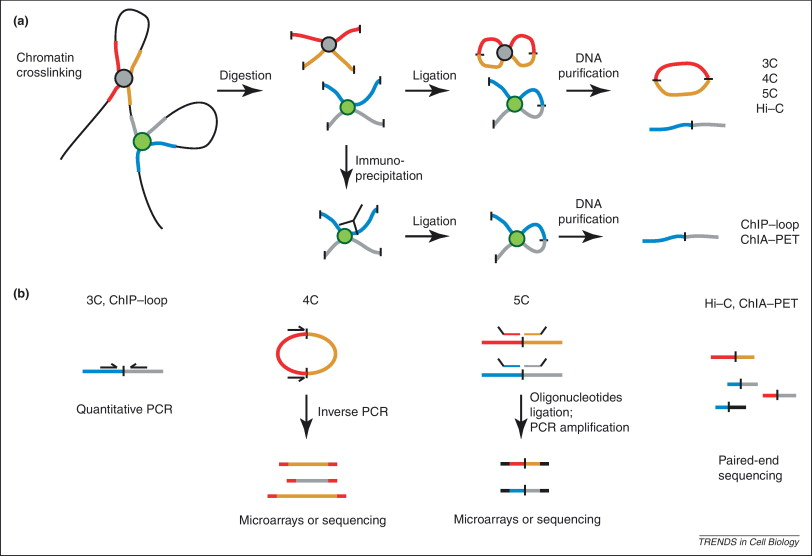
\includegraphics[width=\textwidth]{figures/biology/CompareChromosomeCapture}
  \medskip
  \small
  Chromatin is uniformly cross-linked and digested with a restriction enzyme.
  Bound sequences are immunoprecipitated or biotinylated, depending on the
  assay, and strands are ligated.  Ligation yields novel chimeric sequences
  which are purified.  The number of interactions are assess by qPCR in
  the canonical \gls{3C} method and ChIP-loop, inverse PCR in 4C, multiplexed
  sequencing with oligonucleotides in 5C, and paired end sequencing in Hi-C
  and ChIA-PET\@.  Adapted from Montavon et al. \citep{montavon2012}.
\end{figure}


The perceptive reader will note that much can go wrong in a \gls{3C} experiment. Every \gls{3C} method involves some level of digestion, ligation,
and amplification, and errors may be introduced at each step.  In particular, Dekker provides guidelines for three important control steps to
ensure the methodology remains integrous: control of PCR efficiency, determination of background random collisions and data
normalization \citep{dekker2006}.  Many derivative methods omit the PCR step, however all methodologies must be cognizant that
biases are introduced in any replacement protocol.

\section*{Topology and Fragility}

The first investigations into nuclear architecture were conducted by examining cell karyotypes.  Despite the development of the karyotype as a
tool for examining nuclear material in the early 20th century \citep{levitsky1924}, it wasn't until 1954 that the number of chromosomes in a human
cell were definitely described \citep{tjio1956}.  Early investigations into nuclear architecture, even using simple karyotypes, were
hampered by technical limitations and chromosomal phenomena such as \gls{non-disjunction} and breakage.  It is not surprising that soon after the
initial description the human chromosomal number, Debakan and colleagues characterized common sites where chromosomes would undergo breakage or
translocations.  They termed these regions \gls{CFS} \citep{leyden2008}.

Many particularities render studying fragile sites difficult.  The first difficulty is semantic; chromosomal fragile sites are not precisely
defined in the literature.  When a study is performed that encompasses fragile sites, typically one of three definitions is used: regions
that are particularly sensitive to forming gaps or breaks on metaphase chromosomes \citep{glover2005}, sites where chromatin fails to compact
under mitosis \citep{leyden2008}, and non-randomly distributed loci that exhibit an increased frequency of breakage under replicational
stress \citep{franchitto2013}.  For the purposes of this discussion, a \gls{fragile site} is a region on the chromosome prone to
forming complex rearrangements, particularly double-strand breaks, repeat extensions, and translocations, when subjected to replicational stress.
These rearrangements play a pivotal role in many severely deliberating genetic diseases.

Fragile sites come in two flavors: common fragile sites (CFS) and rare fragile sites (RFS).  Fragile sites are classified into a group based on their
prevalence in the population, and the conditions under which their fragility is induced \citep{leyden2008}.  Common fragile sites are thought to be common
to all humans, while rare fragile sites may be expressed in small fraction (less than 5\%) of the population \citep{wells2006}.

Rearrangements play pivotal roles in severely debilitating genetic diseases such as Fragile X Syndrome.  All males and an estimated that 60\% of females
with repeat anomalies near the FRM1 gene on the X chromosome suffer from severe mental handicap due to these alterations \citep{sutherland1995}. Additionally,
fragile sites are often found rearranged in human cancers \citep{glover2005}.  Despite these findings, the basis of fragility in fragile sites is still an
unanswered question.


% TODO
% Combine this chapter and the biology chapter.
\chapter{Fragility in the Code}

The first investigations into nuclear architecture were conducted by
examining cell karyotypes.  Despite the development of the karyotype as a
tool for examining nuclear material in the early 20th
century\cite{levitsky1924}, it wasn't until 1954 the number of chromosomes in
a human cell were definitely described\cite{tjio1956}.  Early investigations
into nuclear architecture, even at the course level of a karyotype, were
hampered by technical limitations and chromosomal phenomena such as
non-dysjunction and breakage.  It is not surprising that soon after the
initial description the human chromosomal number, Debakan and colleagues
characterized common sites were chromosomes would undergo breakage or
translocations.  They termed these regions
\textit{chromosomal fragile sites}\cite{leyden2008}.

Many particularities render studying fragile sites difficult.  The
first difficulty is semantic; chromosomal fragile sites are not precisely
defined in the literature.  When a study is performed that encompasses fragile
sites, typically one of three definitions is used: regions that are particularly
sensitive to forming gaps or breaks on metaphase chromosomes\cite{glover2005},
sites where chromatin fails to compact under mitosis\cite{leyden2008}, and
non-randomly distributed loci that exhibit an increased frequency of breakage
under replicational stress\cite{franchitto2013}.  For the purposes of this
discussion, a \textit{fragile site} is a region on the chromosome prone to
forming complex rearrangements, particularly double-strand breaks, repeat
extensions, and translocations, when subjected to replicational stress.  These
rearrangements play a pivotal role in many severely deliberating genetic
diseases.

Fragile sites come in two flavors: common fragile sites (CFS) and rare fragile
sites (RFS).  Fragile sites are classified into a group based on their
prevalence in the population, and the conditions under which their fragility
is induced\cite{leyden2008}.  Common fragile sites are thought to be common
most chromosomes and to all humans, while rare fragile sites may be expressed
in small fraction (less than 5\%) of the population\cite{wells2006}.

These
rearrangements play pivotal roles in severely debilitating genetic diseases
such as Fragile X Syndrome.  All males and an estimated that 60\% of females
with repeat anomalies near the FRM1 gene on the X chromosome suffer
from severe mental handicap due to these alterations\cite{sutherland1995}.
Additionally, fragile sites are often found rearranged in human
cancers\cite{glover2005}.  Despite these findings, reason fragile site are
fragile is still an unanswered question.

% CFS's may be epigenetically defined. (Molecular profiling of CFS in human fibroblasts
% CFS are conserved based on cell types

% TODO NOT SURE WHERE THIS GOES

%% Data Validation

%% Iterative Correction and Eigenvalue Expansion

%% Visualization Tools
%% Replication Timing Analysis..?

% results.tex

\chapter{Results \& Discussion}

\section*{The number of interactions is a function of distance and chromosome}
In earlier treatments of the Hi-C data sets, the analysis of folding patterns by various groups\cite{imakaev2012}\cite{dixon2012}
the density of bound probes as a function of distance for the entire genome.  However, in our analysis, we remark that chromosomes
have heterogeneous scaling properties, as seen figure~\ref{fig:interactionScaling}.

\begin{figure}[h]
  \caption{Number of interactions as a function of distance.}\label{fig:interactionScaling}
\end{figure}

We find that the relative ordering of these curves are reproducible between replicates (Pearson=?).  This implies th.

Notably, the scaling ratios are unchanged by normalization, indicating that scaling may be a property of the underlying distribution
rather than an artifact of out data processing.  Indeed, this indicates that perhaps normalization should be performed, as is
done in HiCNorm\cite{hu2012} on a chromosome by chromosome basis, estimating different background distributions for each chromosome
rather than using a generalized fitting algorithm such as IPF\@.  This.

\section*{Differentiation induces fibroblast-specific gene products in IMR90}

The transition from embryonic pluripotency to a specialized cell type naturally introduces a change in the expressed cell products.
Using Affymetrix microarrays, we observe that the overall trend towards differentiation marginally increases gene expression across
the entire proteome (mean=?).  This observation is not surprising, and is thoroughly documented in the literature\cite{tuomela2012}
for various cell types.

We then sought to understand how expression changes were related to molecular function in the cell.  Using the ConsensusPathDB
tool\cite{kamburov2012}, we performed both over expression and gene ontology analysis of the 1\%  largest positively and negatively
and signalling pathways.  Furthermore, downregulated genes are involved in transcriptional regulation of pluripotent stem cells.

We asked whether transcriptional upregulation during differentiation could predict mutations, lesions, or break points seen in lung
cancer studies.  We acquired data for every type of lung cancer lesions from the Catalogue of Somatic Mutations in Cancer
(COSMIC)\cite{forbes2009} by gene.  Interestingly, the frequency of lesions reported by COSMIC was uncorrelated to those genes
expression changes (Pearsons $0.07$, $p < 1 \times 10^{-18}$).  There are a number of potential causes for the lack of signal in
our expression data.  Perhaps the expression arrays are not able to identify gene fusion products, a non-negligible portion of
the COSMIC mutation database.  More likely, as reported recently by Ashworth and colleagues, it is mutations in transcription factors
that cause gene expression changes in cancers, rather than in the genes themselves\cite{ashworth2014}.

\section*{Contact maps of cell lines change drastically during differentiation}
% TODO

\section*{Cancerous lesions are in close proximity to topological domains}


%
% APPENDIX
%

\appendix
\appendixpage
\addappheadtotoc

% appendix.tex
\chapter{Data Collection}

Methylation data was downloaded from the Salk Institute for Biology Studies in
two files from two biological replicates.  Each file contained $\sim600$ million
reads from the

\begin{table}
  \centering
  \begin{tabular}{lccr}
    \hline
    Replicate & Hg18 Reads & Hg19 Reads & Unlifted Reads \\ \hline
    1 & 563,354,527 & 563,071,323 & 566,408 \\
    2 & 620,520,572 & 620,227,842 & 585,460 \\
    \hline
  \end{tabular}
  \caption{Genomic methylation data for IMR90}
\end{table}

\chapter{Data Migration to Human Genome Build 19}

To make valid comparisons between disparate data sets, it is crucial to ensure all data sets are aligned to the same
build of the human genome.  A genome build is a haploid assembly of sequences from several individuals published by
the NCBI to provide a reference for an organism gene and feature set, though not necessarily every allele.  A build assembly
refers to a particular published sequence annotation set.  Human Genome Build 19 (HG19) is the University of California Santa
Cruz nomenclature for the NCBI Build GRCh37 published in 2009\cite{lander2001}.

In this thesis, the methylation and histone assays were all reported against human genome build 18.  Experiments aligned
against previous builds of the human genome may be updated informatically, either by re-alignment of the
sequence probes or through coordinate transposition.  The UCSC Genome Browser provides a command line utility liftOver for
batch coordinate conversion.  Each file was unzipped and updated to HG19 prior to further analysis using the liftOver tool.

\begin{table}
  \centering
  \begin{tabular}{lccr}
    \hline
    Sample & HG18 Reads & HG19 Reads & Unlifted Reads \\ \hline
    H3K27ac & 16374518 & 16371125 & 3,393 \\
    p65 & 16371125 & 6165230 & 947 \\
    H3K4me1 & 18713234 & 18709033 & 4201 \\
    H3K36me3 & 15808706 & 15807726 & 980 \\
    CTCF & 5501307 & 5499946 & 1361 \\
    \hline
  \end{tabular}
  \caption{Genomic methylation data for IMR90}
\end{table}

\chapter{Iterative Alignment of Probes}

Probes were aligned to the human genome build hg19 using procedures outlined by
Imakaev and colleagues\cite{imakaev2012}.  The chimeric nature of the reads
requires that probes be aligned iteratively, starting from a small, truncated
region from the beginning of the read, mapping this truncated area, increasing
the truncation size and recursing a fixed number of steps or until the alignment
scores become sufficiently poor.  Due to the large number of reads requiring
alignment, we opted to use a fixed truncation length (based on sequence length)
and four steps in the iterative alignment protocol.  The calculation
for the truncation and step size can be found in the the iterativeMapping.py
script provided in the Appendix: Code.  Most reads were 100 base pairs, resulting
in an initial truncation length of 28 base pairs, and step size of 18 base pairs.

Using the mapping functionality from the hiclib python package\cite{imakaev2012},
sequences from the six experimental replicates were realigned to the genome.  The
alignment employed the fast Bowtie2 alignment algorithm\cite{langmead2012}.  Once
aligned, the probes were stored as an interaction matrix in the high performance
HDF5\cite{hdf5} data format, a total of 25Gb for all replicates.

Statistics for iterative alignment are given below:

\begin{center}
  \begin{table}
    \begin{tabular}{l l}
    Total Reads & 2,124,453,478 \\
    Total DS Reads & 1,422,870,270 \\
    Valid Pairs & 713,897,554 \\
    Filtered Reads & 457,298,174 \\
    Percent \textit{trans} Reads & 49.42\% \\
    \end{tabular}
  \end{table}
\end{center}


\chapter{Data Validation}

In order to make meaningful comparisons between data sets (replicates,
in this case), we must show that some degree of relationship exists between
the data sets and comparisons or combinations of the data from disparate sets
are valid to a degree of uncertainty.  It is also essential to understand if the
experimental replicates indeed managed to replicate the conditions of the primary
experiment, or if experimental errors prevent the comparison between replicates.

Spearman's Rank Correlation Coefficient (denoted by the Greek letter $\rho$) is
a non-parametric measure of association between two variables.
Spearman's coefficient assumes some monotonic relationship between variables,
rather than a linear relationship (as in Pearson's), making it appropriate
to compare the IMR90 interaction data sets.  The formula for Spearman's $\rho$ is
given as follows:

\begin{equation}
\rho = 1 - \frac{\sum_{i=1}{n}(d_i^2)}{n(n^2 - 1)}
\end{equation}

where $\rho$ is the correlation coefficient taking values between $-1$ and $+1$,
$d_i = x_i - y_i$ where $x_i, y_i$ are ranks derived from the raw scores $X$ and
$Y$ respectively.

The first replicate IMR90 interaction data set was labeled the primary data set
and the remaining five were compared using Spearman's Rank Correlation.  The
results are given in Table X.

\begin{table}
  \begin{tabular}{|c|*{6}{c|}}
    \toprule
    \textbf{R1} & 0.83 & 0.77 & 0.77 & 0.75 & 0.71 \\ \midrule
    0.83 & \textbf{R2} & 0.82 & 0.83 & 0.79 & 0.75 \\ \midrule
    0.77 & 0.82 & \textbf{R3} & 0.77 & 0.74 & 0.73 \\ \midrule
    0.77 & 0.83 & 0.77 & \textbf{R4} & 0.75 & 0.71 \\ \midrule
    0.75 & 0.79 & 0.74 & 0.74 & \textbf{R5} & 0.69 \\ \midrule
    0.71 & 0.75 & 0.73 & 0.71 & 0.69 & \textbf{R6} \\ \midrule
  \end{tabular}
  \caption{Spearman's $\rho$ across all data sets.}
\label{tab:correlations}
\end{table}


%
% Glossary
%
% Acronym Definitions
\setacronymstyle{long-short}

% Biology
\newacronym[description=any of various nucleic acids that are usually the molecular basis of heredity]
{DNA}{DNA}{deoxyribonucleic acid}

\newacronym{TCGA}{TCGA}{The Cancer Genome Atlas}

\newacronym[description=any of various nucleic acids that are usually the molecular basis of heredity]
{bp}{bp}{base pair}

\newacronym[description=any of various nucleic acids that contain ribose and uracil as structural components and are associated with the control of cellular chemical activities—called also ribonucleic acid]
{RNA}{RNA}{ribonucleic acid}

\newacronym[description=the Gene Expression Omnibus.  Located at \url{http://www.ncbi.nlm.nih.gov/geo/}]{GEO}{GEO}{Gene Expression Omnibus}

\newacronym[description=the National Center for Biotechnology Information.  Located at \url{http://www.ncbi.nlm.nih.gov/}]
{NCBI}{NCBI}{National Center for Biotechnology Information}

\newacronym[description=stores raw sequencing data and alignment information from high-throughput sequencing platforms.  For more information see \url{http://www.ncbi.nlm.nih.gov/sra}]
{SRA}{SRA}{Sequence Read Archive}

\newacronym[description=local regions of highly enriched chromatin interactions]
{TAD}{TAD}{Topologically Associating Domain}

\newacronym[description=genome-lamina interacting domains found to be 0.1--10 megabases in size]
{LAD}{LAD}{Lamina Associated Domain}

\newacronym{DS}{DS}{double-stranded}

\newacronym{GC}{GC}{guanine-cytosine}

\newacronym[description=human embryonic stem cell line cultured in lab]
{hESC}{hESC}{Human embryonic stem cell}

\newacronym[description=the location where transcription starts at the 5'-end of a gene sequence]
{TSS}{TSS}{Transcriptional Start Site}

\newacronym[
  \glsshortpluralkey={GTFs},
  description=a class of protein transcription factors that bind to specific sites (promoter) on DNA to activate transcription of genetic information from DNA to messenger RNA
]{GTF}{GTF}{General Transcription Factor}

\newacronym{PIC}{PIC}{preinitiation complex}

\newacronym[longplural={chromosome territories}]{CT}{CT}{chromosome territory}

\newacronym{3C}{3C}{Chromosome Conformation Capture}

\newacronym{4C}{4C}{Chromosome Conformation Capture-on-Chip}

\newacronym{5C}{5C}{Chromosome Conformation Capture Carbon-Copy}

\newacronym{NGS}{NGS}{Next Generation Sequencing}

\newacronym{COSMIC}{COSMIC}{The Catalogue of Somatic Mutations in Cancer}

\newacronym[description=a function of a continuous random variable whose integral across an interval gives the probability that the value of the variable lies within the same interval]
{pdf}{pdf}{probability density function}

\newacronym[description=a specific heritable point on a chromosome that tends to form a gap or constriction and may tend to break when the cell is exposed to partial replication stress]
{CFS}{CFS}{chromosome fragile site}


% maths
\newacronym{PCA}{PCA}{Principal Component Analysis}
\newacronym{SVD}{SVD}{Singular Value Decomposition}
\newacronym[
  \glsshortpluralkey={PCs},
]{PC}{PC}{principal component}
\newacronym{ICE}{ICE}{Iterative Correction and Eigenvector Decomposition}
\newacronym{DI}{DI}{Directionality Index}

\newacronym{EM}{EM}{expectation maximization}

\newacronym[description=A proceedure for adjusting a table of data cells such that they add up to selected totals for both columns and rows (in the two dimensional case) of the table]
{IPF}{IPF}{iterative proportional fitting}

\newacronym[description=A technique, given an observed ]
{MLE}{MLE}{maximum likelihood estimation}

\newacronym{HMM}{HMM}{hidden markov model}

% Glossary definitions
\newglossaryentry{karyotype}{%
  name={karyotype},
  description={a photomicrograph of chromosomes arranged according to a standard classification}%
}

\newglossaryentry{trans contact}{%
  name={\textit{trans} contact},
  plural={\textit{trans} contacts},
  description={interactions that occur between bins on two different chromosomes}%
}

\newglossaryentry{cis contact}{%
  name={\textit{cis} contact},
  plural={\textit{cis} contacts},
  description={interactions that occur between bins on the same chromosome}%
}

\newglossaryentry{contact map}{%
  name={contact map},
  description={a non-negative, square matrix recording observed interactions between different genomic regions}%
}

\newglossaryentry{nucleobase}{%
  name={nucleobase},
  description={nitrogen-containing biological compounds (nitrogenous bases) found linked to a sugar within nucleosides—the basic building blocks of deoxyribonucleic acid (DNA) and ribonucleic acid (RNA). B substance that has a molecular structure consisting chiefly or entirely of a large number of similar units bonded together, e.g., many synthetic organic materials used as plastics and resins}
}

\newglossaryentry{polymer}{%
  name={Polymer},
  description={a substance that has a molecular structure consisting chiefly or entirely of a large number of similar units bonded together, e.g., many synthetic organic materials used as plastics and resins}
}

\newglossaryentry{epigenetic}{%
  name={epigenetic},
  description={any heritable influence on gene activity, unaccompanied by a change in the DNA}
}

\newglossaryentry{restriction enzyme}{%
  name={restriction enzyme},
  description={an enzyme that restricts, or performs double-strand cut, at a specific DNA sequence motif}
}

\newglossaryentry{ligation}{%
  name={ligation},
  description={the joining of two DNA strands or other molecules by a phosphate ester linkage}
}

\newglossaryentry{nucleotide}{%
  name={nucleotide},
  description={a compound consisting of a nucleoside linked to a phosphate group. Nucleotides form the basic structural unit of nucleic acids such as DNA}
}

\newglossaryentry{oligonucleotide}{%
  name={oligonucleotide},
  description={a polynucleotide whose molecules contain a relatively small number of nucleotides}
}

\newglossaryentry{nucleosome}{%
  name={nucleosome},
  description={a chromatin secondary structure consisting of $\sim147$ base pairs of DNA wrapped 1.75 times around an octamer of core histone proteins}
}

\newglossaryentry{scree plot}{%
  name={scree plot},
  description={a graph displaying the eigenvalue associated with each component in descending order versus the component number.  Used in PCA to determine how many components to consider in the analysis}
}

\newglossaryentry{eigenspectrum}{%
  name={eigenspectrum},
  description={a spectrum of eigenvalues}
}

\newglossaryentry{normalization}{%
  name={normalization},
  description={an attempt to compensate for noise and systematic bias from in a particular data set, while preserving the differences in a data set}
}

\newglossaryentry{toric model}{%
  name={toric model},
  description={a background model for a distribution.  Also known as a log-linear model}
}

\newglossaryentry{log-linear}{%
  name={log-linear},
  description={see toric model}
}

\newglossaryentry{transcriptome}{%
  name={transcriptome},
  description={the sum total of all messenger RNA molecules expressed from genes of an organism}
}

\newglossaryentry{contingency table}{%
  name={contingency table},
  description={a type of table in statistics that displays the frequency distribution of variables.  Also called a crosstab}
}

\newglossaryentry{sufficient statistic}{%
  name={sufficient statistic},
  description={a statistic that does as good a job estimating an unknown parameter as the entire sample}
}

\newglossaryentry{norm}{%
  name={norm},
  description={in linear algebra, functional analysis and related areas of mathematics, a function that assigns a strictly positive length or size to each vector in a vector space—save possibly for a single zero vector, with length zero}
}

\newglossaryentry{X-inactivation}{%
  name={x-inactivation},
  description={a process by which one of the two copies of the X chromosome present in female mammals is inactivated}
}

\newglossaryentry{in vivo}{%
  name={in vivo},
  description={performed or taking place in a living organism}
}

\newglossaryentry{nucleosome array}{%
  name={nucleosome array},
  description={the fundamental building block of chromosomal superstructures, the substrate for transcription, and the first nucleoprotein assembly laid down after DNA replication}
}

\newglossaryentry{euchromatin}{%
  name={euchromatin},
  plural={euchromatin},
  description={a lightly packed form of chromatin (DNA, RNA and protein) that is rich in gene concentration, and is often (but not always) under active transcription}
}

\newglossaryentry{heterochromatin}{%
  name={heterochromatin},
  plural={heterochromatin},
  description={chromosome material of different density from normal (usually greater), in which the activity of the genes is modified or suppressed}
}

\newglossaryentry{preinitiation complex}{%
  name={preinitiation complex},
  plural={preinitiation complexes},
  description={large complex of promoter-bound proteins that is necessary for the transcription of protein-coding genes in eukaryotes}
}

\newglossaryentry{high-throughput}{%
  name={high-throughput},
  description={the use of automation equipment with classical cell biology techniques to address biological questions that are otherwise unattainable using conventional methods}
}

\newglossaryentry{fragile site}{%
  name={fragile site},
  description={heritable-specific loci on human chromosomes that exhibit nonrandom gaps or breaks when chromosomes are exposed to specific cell culture conditions}
}

\newglossaryentry{core promoter}{%
  name={core promoter},
  description={the minimal portion of the promoter required to properly initiate gene transcription}
}

\newglossaryentry{variance}{%
  name={variance},
  description={measurement of how far a set of numbers is spread out}
}


%
% BIBLIOGRAPHY
%

\bibliography{bibliography}{}
\bibliographystyle{plos2015}

\printglossaries

\end{document}
